\documentclass[11pt,a4paper]{article}

\usepackage[T1]{fontenc}
\usepackage[utf8]{inputenc}
\usepackage{lmodern}
\usepackage[a4paper,margin=22mm,headheight=15pt]{geometry}
\usepackage{microtype}
\usepackage{amsmath,amssymb,mathtools,bm}
\usepackage{booktabs,array,tabularx}
\usepackage{enumitem}
\usepackage{xcolor}
\usepackage{tikz}
\usetikzlibrary{arrows.meta,calc,positioning}
\usepackage[most]{tcolorbox}
\usepackage{fancyhdr}
\usepackage{titlesec}
\usepackage{hyperref}

\definecolor{ink}{HTML}{17324D}
\definecolor{blue}{HTML}{176B87}
\definecolor{teal}{HTML}{2A9D8F}
\definecolor{gold}{HTML}{E9A23B}
\definecolor{red}{HTML}{C84C4C}
\definecolor{softblue}{HTML}{EAF4F8}
\definecolor{softgold}{HTML}{FFF6E6}
\definecolor{softgreen}{HTML}{EAF7F3}

\hypersetup{
  colorlinks=true,
  linkcolor=blue,
  urlcolor=blue,
  pdftitle={The Laplacian in Spherical Coordinates: An Extremely Slow Derivation},
  pdfauthor={A step-by-step field-calculus tutorial}
}

\pagestyle{fancy}
\fancyhf{}
\fancyhead[L]{\small\color{ink}The spherical Laplacian}
\fancyhead[R]{\small\color{blue}An extremely slow derivation}
\fancyfoot[C]{\small\color{ink}\thepage}
\renewcommand{\headrulewidth}{0.4pt}
\renewcommand{\headrule}{\hbox to\headwidth{\color{blue}\leaders\hrule height \headrulewidth\hfill}}

\titleformat{\section}{\Large\bfseries\color{ink}}{\color{blue}\thesection}{0.7em}{}
\titleformat{\subsection}{\large\bfseries\color{ink}}{\color{teal}\thesubsection}{0.7em}{}
\titlespacing*{\section}{0pt}{1.2em}{0.6em}
\titlespacing*{\subsection}{0pt}{1em}{0.4em}

\setlength{\parindent}{0pt}
\setlength{\parskip}{0.55em}
\setlist[itemize]{leftmargin=1.5em,itemsep=0.3em,topsep=0.3em}
\setlist[enumerate]{leftmargin=1.7em,itemsep=0.4em,topsep=0.3em}

\newcommand{\er}{\bm e_r}
\newcommand{\etheta}{\bm e_\theta}
\newcommand{\ephi}{\bm e_\phi}
\newcommand{\dd}{\mathop{}\!\mathrm d}

\newtcolorbox{idea}[1][]{
  enhanced,breakable,colback=softblue,colframe=blue,
  boxrule=0.7pt,arc=2mm,left=3mm,right=3mm,top=2mm,bottom=2mm,
  title={#1},fonttitle=\bfseries,coltitle=ink
}
\newtcolorbox{notecheck}[1][]{
  enhanced,breakable,colback=softgold,colframe=gold,
  boxrule=0.7pt,arc=2mm,left=3mm,right=3mm,top=2mm,bottom=2mm,
  title={#1},fonttitle=\bfseries,coltitle=ink
}
\newtcolorbox{result}[1][]{
  enhanced,breakable,colback=softgreen,colframe=teal,
  boxrule=0.9pt,arc=2mm,left=3mm,right=3mm,top=2mm,bottom=2mm,
  title={#1},fonttitle=\bfseries,coltitle=ink
}

\begin{document}

\begin{titlepage}
\thispagestyle{empty}
\vspace*{12mm}
{\color{blue}\rule{\textwidth}{1.2pt}}

\vspace{10mm}
{\Huge\bfseries\color{ink}The Laplacian in Spherical Coordinates\par}
\vspace{4mm}
{\LARGE\color{blue}An extremely slow derivation\par}
\vspace{6mm}
{\large\color{ink}From tiny arc lengths to $\nabla^2 f$, with every geometric factor explained\par}

\vspace{13mm}
\begin{center}
\begin{tikzpicture}[scale=1.02,>=Latex]
  \coordinate (O) at (0,0);
  \coordinate (P) at (4.35,3.55);
  \coordinate (H) at (4.35,0);
  \draw[->,ink!60] (-0.45,0) -- (5.9,0) node[right] {$x$};
  \draw[->,ink!60] (0,-0.35) -- (0,4.9) node[above] {$z$};
  \draw[->,ink!60] (0,0) -- (-1.85,-1.05) node[below left] {$y$};
  \draw[ink!30,dashed] (P) -- (H);
  \draw[->,blue,line width=2pt] (O) -- (P) node[pos=0.55,above left] {$r$};
  \draw[teal,line width=1.5pt] (O) -- (H) node[midway,below] {$r\sin\theta$};
  \fill[ink] (P) circle (2.2pt);
  \draw[red,->] (0,1.12) arc[start angle=90,end angle=39.2,radius=1.12];
  \node[red] at (0.53,1.00) {$\theta$};
  \draw[gold,->] (1.25,0) arc[start angle=0,end angle=-29,radius=1.25];
  \node[gold!80!black] at (1.45,-0.34) {$\phi$};
  \node[anchor=west,text width=5.3cm,align=left,color=ink] at (6.45,2.45)
  {Every factor will come from a visible length or area:\\[1mm]
   \textcolor{blue}{$\dd r$},\quad
   \textcolor{teal}{$r\,\dd\theta$},\quad
   \textcolor{gold!80!black}{$r\sin\theta\,\dd\phi$}.};
\end{tikzpicture}
\end{center}

\vfill
\begin{idea}[The plan]
First find three tiny physical distances. Use them to derive the gradient. Then build the divergence by measuring flux through the six faces of a tiny spherical box. Finally set the vector field equal to the gradient. Nothing is quoted as a mysterious coordinate formula.
\end{idea}

\vspace{8mm}
{\small\color{ink!75}Convention: $\theta$ is measured down from the positive $z$-axis; $\phi$ turns around the $z$-axis.\par}
\vspace{7mm}
{\color{blue}\rule{\textwidth}{1.2pt}\par}
\end{titlepage}

\setcounter{tocdepth}{1}
\tableofcontents
\thispagestyle{fancy}
\clearpage

\section{What we are trying to derive}

Let \(f=f(r,\theta,\phi)\) be a smooth scalar field. It might be temperature, pressure, concentration, or potential. Our target is the spherical-coordinate form of
\[
  \nabla^2f=\nabla\cdot(\nabla f).
\]

The final expression contains several factors of \(r\) and \(\sin\theta\). Instead of memorising them, we will account for each one geometrically.

\begin{idea}[Physical meaning]
The gradient tells us how \(f\) rises with physical distance. The divergence of that gradient measures the net outward gradient flux per unit volume. Thus the Laplacian compares a value with the values around it.
\end{idea}

The derivation has four stages:
\begin{enumerate}
  \item find the lengths corresponding to \(\dd r\), \(\dd\theta\), and \(\dd\phi\);
  \item derive \(\nabla f\) from \(\dd f=\nabla f\cdot\dd\bm\ell\);
  \item derive \(\nabla\cdot\bm A\) from flux divided by volume;
  \item substitute \(\bm A=\nabla f\).
\end{enumerate}

\subsection{Fix the convention before doing algebra}

We use the convention common in physics:
\begin{itemize}
  \item \(r\geq0\) is distance from the origin;
  \item \(0\leq\theta\leq\pi\) is measured down from \(+z\);
  \item \(0\leq\phi<2\pi\) is measured around the \(z\)-axis from \(+x\).
\end{itemize}
Therefore
\begin{align*}
  x&=r\sin\theta\cos\phi,\\
  y&=r\sin\theta\sin\phi,\\
  z&=r\cos\theta.
\end{align*}

At every ordinary point we attach three mutually perpendicular unit vectors:
\[
  \er,\qquad\etheta,\qquad\ephi.
\]
They point in the directions of increasing \(r\), increasing \(\theta\), and increasing \(\phi\).

\begin{notecheck}[Notation warning]
Some books exchange the names \(\theta\) and \(\phi\). Always check which angle is measured from the \(z\)-axis. A swapped convention gives a formula that looks different even though the geometry is the same.
\end{notecheck}

\clearpage

\section{Three coordinate changes, three physical lengths}

The symbols \(\dd r\), \(\dd\theta\), and \(\dd\phi\) are coordinate changes. Only \(\dd r\) is already a physical length. An angle change must be multiplied by the radius of the circle along which the point moves.

\subsection{Radial step: change \(r\), hold both angles fixed}

The point moves straight outward. A small increase \(\dd r\) gives
\[
  \dd\bm\ell_r=\dd r\,\er.
\]
Its physical length is simply
\[
  \boxed{\dd\ell_r=\dd r}.
\]

The scale factor is the physical length per unit coordinate change:
\[
  h_r=\frac{\dd\ell_r}{\dd r}=1.
\]

\subsection{Polar step: change \(\theta\), hold \(r\) and \(\phi\) fixed}

The point moves along a meridian. This is a circle of radius \(r\), centred at the origin.

For an angle measured in radians,
\[
  \text{arc length}
  =(\text{circle radius})(\text{angle change}).
\]
Therefore
\[
  \dd\bm\ell_\theta=r\,\dd\theta\,\etheta,
  \qquad
  \boxed{\dd\ell_\theta=r\,\dd\theta}.
\]
The scale factor is
\[
  h_\theta=\frac{\dd\ell_\theta}{\dd\theta}=r.
\]

\subsection{Azimuthal step: change \(\phi\), hold \(r\) and \(\theta\) fixed}

The point moves around the \(z\)-axis on a circle of latitude. We must first find the radius of that circle.

In a meridional right triangle, the hypotenuse is \(r\) and the side perpendicular to the \(z\)-axis is
\[
  \rho=r\sin\theta.
\]
Thus the azimuthal circle has radius \(r\sin\theta\), not \(r\). The arc length is
\[
  \dd\bm\ell_\phi
  =r\sin\theta\,\dd\phi\,\ephi,
  \qquad
  \boxed{\dd\ell_\phi=r\sin\theta\,\dd\phi}.
\]
The scale factor is
\[
  h_\phi=\frac{\dd\ell_\phi}{\dd\phi}=r\sin\theta.
\]

\begin{center}
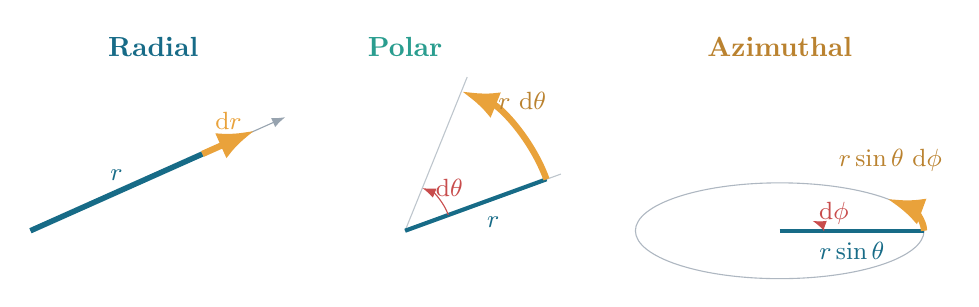
\begin{tikzpicture}[scale=0.78,>=Latex,font=\small]
  \begin{scope}[xshift=-6.1cm]
    \node[font=\bfseries,color=blue] at (2.0,3.0) {Radial};
    \coordinate (O) at (0,0);
    \coordinate (P) at (2.8,1.25);
    \coordinate (Q) at (3.65,1.63);
    \draw[->,ink!45] (O) -- (4.15,1.85);
    \draw[blue,line width=2pt] (O) -- (P) node[midway,above] {$r$};
    \draw[->,gold,line width=2.3pt] (P) -- (Q) node[midway,above] {$\dd r$};
  \end{scope}

  \begin{scope}
    \node[font=\bfseries,color=teal] at (0,3.0) {Polar};
    \coordinate (O) at (0,0);
    \draw[ink!28] (O) -- (20:2.7);
    \draw[ink!28] (O) -- (68:2.7);
    \draw[blue,line width=1.5pt] (O) -- (20:2.45) node[midway,below right] {$r$};
    \draw[gold,line width=2.3pt,->] (20:2.45) arc[start angle=20,end angle=68,radius=2.45];
    \draw[red,->] (20:0.75) arc[start angle=20,end angle=68,radius=0.75];
    \node[red] at (44:1.0) {$\dd\theta$};
    \node[gold!80!black] at (48:2.85) {$r\,\dd\theta$};
  \end{scope}

  \begin{scope}[xshift=6.1cm]
    \node[font=\bfseries,color=gold!80!black] at (0,3.0) {Azimuthal};
    \draw[ink!35] (0,0) ellipse (2.35 and 0.78);
    \draw[blue,line width=1.5pt] (0,0) -- (2.35,0)
      node[midway,below] {$r\sin\theta$};
    \draw[gold,line width=2.3pt,->]
      (2.35,0) arc[start angle=0,end angle=42,x radius=2.35,y radius=0.78];
    \draw[red,->] (0.72,0) arc[start angle=0,end angle=42,x radius=0.72,y radius=0.24];
    \node[red] at (0.88,0.29) {$\dd\phi$};
    \node[gold!80!black] at (1.8,1.15) {$r\sin\theta\,\dd\phi$};
  \end{scope}
\end{tikzpicture}
\end{center}

\clearpage

\section{Collect the geometry}

The three independent steps combine to give the tiny displacement
\begin{result}[Spherical line element]
\[
  \boxed{
  \dd\bm\ell
  =\dd r\,\er
  +r\,\dd\theta\,\etheta
  +r\sin\theta\,\dd\phi\,\ephi.}
\]
Because the three directions are perpendicular,
\[
  \boxed{
  \dd\ell^2
  =\dd r^2+r^2\dd\theta^2
  +r^2\sin^2\theta\,\dd\phi^2.}
\]
\end{result}

The scale factors are therefore
\[
  \boxed{h_r=1,\qquad h_\theta=r,\qquad h_\phi=r\sin\theta.}
\]

\begin{center}
\renewcommand{\arraystretch}{1.3}
\begin{tabularx}{0.94\textwidth}{>{\bfseries}c X c c}
\toprule
Change & Curve followed & Physical length & Scale factor\\
\midrule
$\dd r$ & straight radial line & $\dd r$ & $h_r=1$\\
$\dd\theta$ & meridian circle of radius $r$ & $r\,\dd\theta$ & $h_\theta=r$\\
$\dd\phi$ & latitude circle of radius $r\sin\theta$ & $r\sin\theta\,\dd\phi$ & $h_\phi=r\sin\theta$\\
\bottomrule
\end{tabularx}
\end{center}

\begin{notecheck}[A pole check]
Near either pole, \(\sin\theta\) is small. Turning through a fixed \(\dd\phi\) moves the point only a small distance. At a pole, \(\sin\theta=0\), so changing \(\phi\) does not move the point at all. At the equator, \(\sin\theta=1\), so the azimuthal circle has radius \(r\).
\end{notecheck}

\subsection{The tiny volume}

A sufficiently small spherical coordinate cell looks locally like a rectangular box. Its perpendicular edge lengths are
\[
  \dd r,\qquad r\,\dd\theta,\qquad r\sin\theta\,\dd\phi.
\]
Multiply them:
\begin{result}[Tiny spherical volume]
\[
  \boxed{
  \dd V
  =(\dd r)(r\,\dd\theta)(r\sin\theta\,\dd\phi)
  =r^2\sin\theta\,\dd r\,\dd\theta\,\dd\phi.}
\]
\end{result}

This volume will be the denominator in the divergence calculation.

\clearpage

\section{Derive the gradient}

Let \(f=f(r,\theta,\phi)\). Its ordinary total differential is
\[
  \dd f
  =\frac{\partial f}{\partial r}\dd r
  +\frac{\partial f}{\partial\theta}\dd\theta
  +\frac{\partial f}{\partial\phi}\dd\phi.
\]
This describes change per coordinate increment. The gradient must describe change per physical distance.

\subsection{Use the defining property}

The gradient is defined by
\[
  \dd f=\nabla f\cdot\dd\bm\ell.
\]
Write its unknown components as
\[
  \nabla f=G_r\er+G_\theta\etheta+G_\phi\ephi.
\]
Now insert the line element:
\begin{align*}
  \dd f
  &=(G_r\er+G_\theta\etheta+G_\phi\ephi)\cdot\\
  &\quad(\dd r\,\er+r\,\dd\theta\,\etheta
  +r\sin\theta\,\dd\phi\,\ephi).
\end{align*}

Because the basis is orthonormal, equal directions have dot product \(1\) and different directions have dot product \(0\). Thus
\[
  \dd f
  =G_r\dd r+G_\theta r\,\dd\theta
  +G_\phi r\sin\theta\,\dd\phi.
\]

The coordinate changes are independent. Their coefficients must match those in the ordinary total differential.

\subsubsection*{Match the coefficient of \(\dd r\)}

\[
  G_r=\frac{\partial f}{\partial r}.
\]

\subsubsection*{Match the coefficient of \(\dd\theta\)}

\[
  rG_\theta=\frac{\partial f}{\partial\theta}
  \quad\Longrightarrow\quad
  G_\theta=\frac{1}{r}\frac{\partial f}{\partial\theta}.
\]

\subsubsection*{Match the coefficient of \(\dd\phi\)}

\[
  r\sin\theta\,G_\phi=\frac{\partial f}{\partial\phi}
  \quad\Longrightarrow\quad
  G_\phi=\frac{1}{r\sin\theta}\frac{\partial f}{\partial\phi}.
\]

Therefore
\begin{result}[Gradient in spherical coordinates]
\[
  \boxed{
  \nabla f
  =\frac{\partial f}{\partial r}\er
  +\frac{1}{r}\frac{\partial f}{\partial\theta}\etheta
  +\frac{1}{r\sin\theta}\frac{\partial f}{\partial\phi}\ephi.}
\]
\end{result}

\begin{idea}[The reciprocal factors are physical]
\(\partial f/\partial\theta\) is change per radian. One radian in the \(\theta\) direction spans physical distance \(r\), so change per unit length is \((1/r)\partial f/\partial\theta\). Similarly, one radian in the \(\phi\) direction spans \(r\sin\theta\).
\end{idea}

If \(f\) has units \([f]\), every gradient component has units \([f]/L\).

\section{Prepare the six flux faces}

Let
\[
  \bm A=A_r\er+A_\theta\etheta+A_\phi\ephi
\]
be a vector field. Divergence is net outward flux per unit volume:
\[
  \nabla\cdot\bm A
  =\lim_{\Delta V\to0}
  \frac{\text{outward flux through the boundary}}{\Delta V}.
\]

We use a tiny cell with coordinate widths \(\dd r,\dd\theta,\dd\phi\).

\begin{center}
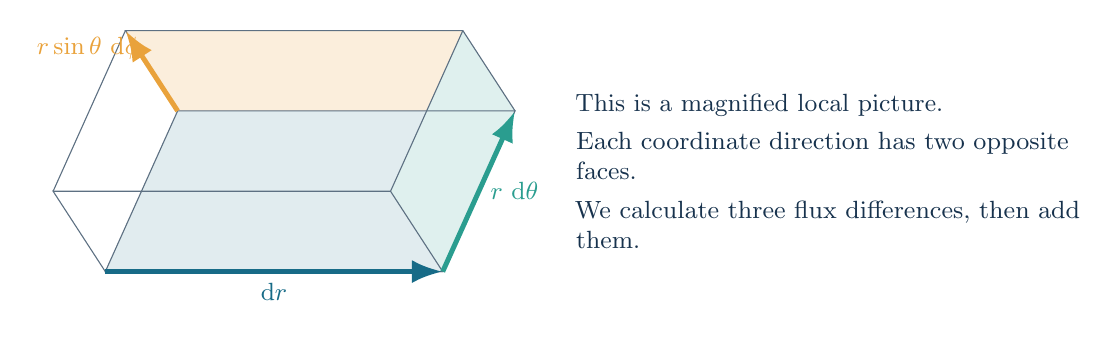
\begin{tikzpicture}[scale=1.02,>=Latex,font=\small]
  \coordinate (O) at (0,0);
  \coordinate (R) at (4.2,0);
  \coordinate (T) at (0.9,2.0);
  \coordinate (P) at (-0.65,1.0);
  \coordinate (RT) at ($(R)+(T)$);
  \coordinate (RP) at ($(R)+(P)$);
  \coordinate (TP) at ($(T)+(P)$);
  \coordinate (RTP) at ($(R)+(T)+(P)$);
  \fill[blue!13] (O)--(R)--(RT)--(T)--cycle;
  \fill[gold!18] (T)--(RT)--(RTP)--(TP)--cycle;
  \fill[teal!15] (R)--(RP)--(RTP)--(RT)--cycle;
  \draw[ink!70] (O)--(R)--(RT)--(T)--cycle;
  \draw[ink!70] (O)--(P)--(RP)--(R)--cycle;
  \draw[ink!70] (T)--(TP)--(RTP)--(RT);
  \draw[ink!70] (P)--(TP);
  \draw[ink!70] (RP)--(RTP);
  \draw[->,blue,line width=1.8pt] (O) -- (R) node[midway,below] {$\dd r$};
  \draw[->,teal,line width=1.8pt] (R) -- (RT) node[midway,right] {$r\,\dd\theta$};
  \draw[->,gold,line width=1.8pt] (T) -- (TP)
    node[midway,above left] {$r\sin\theta\,\dd\phi$};
  \node[align=left,text width=6.4cm,color=ink] at (9.0,1.25)
  {This is a magnified local picture.\\[1mm]
   Each coordinate direction has two opposite faces.\\[1mm]
   We calculate three flux differences, then add them.};
\end{tikzpicture}
\end{center}

\subsection{Face areas from edge lengths}

A face normal to \(\er\) uses the other two edge lengths:
\[
  \boxed{\dd S_r
  =(r\,\dd\theta)(r\sin\theta\,\dd\phi)
  =r^2\sin\theta\,\dd\theta\,\dd\phi.}
\]

A face normal to \(\etheta\) uses the radial and azimuthal edges:
\[
  \boxed{\dd S_\theta
  =(\dd r)(r\sin\theta\,\dd\phi)
  =r\sin\theta\,\dd r\,\dd\phi.}
\]

A face normal to \(\ephi\) uses the radial and polar edges:
\[
  \boxed{\dd S_\phi
  =(\dd r)(r\,\dd\theta)
  =r\,\dd r\,\dd\theta.}
\]

The field component normal to a face is the only component that crosses that face.

\clearpage

\section{Radial flux pair}

The inner radial face is at \(r\). Its outward normal is \(-\er\), so its flux enters with a minus sign:
\[
  -A_r(r,\theta,\phi)\,
  r^2\sin\theta\,\dd\theta\,\dd\phi.
\]

The outer radial face is at \(r+\dd r\). Its outward normal is \(+\er\). Both the field and the area are evaluated at the larger radius:
\[
  A_r(r+\dd r,\theta,\phi)\,
  (r+\dd r)^2\sin\theta\,\dd\theta\,\dd\phi.
\]

Subtract inner from outer:
\begin{align*}
  \dd\Phi_r
  ={}&\Big[(r+\dd r)^2A_r(r+\dd r,\theta,\phi)
  -r^2A_r(r,\theta,\phi)\Big]\\
  &\times\sin\theta\,\dd\theta\,\dd\phi.
\end{align*}

The bracket is a small change in the single quantity \(r^2A_r\). By the definition of a derivative,
\[
  (r+\dd r)^2A_r(r+\dd r)-r^2A_r(r)
  =\frac{\partial}{\partial r}(r^2A_r)\dd r
\]
to first order. Therefore
\begin{result}[Net radial flux]
\[
  \boxed{
  \dd\Phi_r
  =\frac{\partial}{\partial r}(r^2A_r)
   \sin\theta\,\dd r\,\dd\theta\,\dd\phi.}
\]
\end{result}

\begin{notecheck}[Why \(r^2\) remains inside the derivative]
The outer radial face is larger than the inner face. Even if \(A_r\) is unchanged, more flux can cross the larger face. Differentiating \(r^2A_r\) includes both the change in field strength and the change in area.
\end{notecheck}

Divide this flux by the tiny volume:
\begin{align*}
  \frac{\dd\Phi_r}{\dd V}
  &=
  \frac{
  \frac{\partial}{\partial r}(r^2A_r)
  \sin\theta\,\dd r\,\dd\theta\,\dd\phi
  }{
  r^2\sin\theta\,\dd r\,\dd\theta\,\dd\phi
  }\\
  &=\boxed{
  \frac{1}{r^2}\frac{\partial}{\partial r}(r^2A_r)}.
\end{align*}

\clearpage

\section{Polar-angle flux pair}

The lower polar face is at \(\theta\). Its outward normal is \(-\etheta\). Its flux contribution is
\[
  -A_\theta(r,\theta,\phi)\,
  r\sin\theta\,\dd r\,\dd\phi.
\]

The upper face is at \(\theta+\dd\theta\), with outward normal \(+\etheta\):
\[
  A_\theta(r,\theta+\dd\theta,\phi)\,
  r\sin(\theta+\dd\theta)\,\dd r\,\dd\phi.
\]

Subtract lower from upper:
\begin{align*}
  \dd\Phi_\theta
  ={}&r\Big[
  \sin(\theta+\dd\theta)A_\theta(r,\theta+\dd\theta,\phi)\\
  &\qquad-\sin\theta A_\theta(r,\theta,\phi)
  \Big]\dd r\,\dd\phi.
\end{align*}

The bracket is a small change in \(\sin\theta A_\theta\):
\[
  \sin(\theta+\dd\theta)A_\theta(\theta+\dd\theta)
  -\sin\theta A_\theta(\theta)
  =
  \frac{\partial}{\partial\theta}
  (\sin\theta A_\theta)\dd\theta.
\]
Thus
\begin{result}[Net polar-angle flux]
\[
  \boxed{
  \dd\Phi_\theta
  =r\frac{\partial}{\partial\theta}
  (\sin\theta A_\theta)
  \dd r\,\dd\theta\,\dd\phi.}
\]
\end{result}

Divide by the tiny volume:
\begin{align*}
  \frac{\dd\Phi_\theta}{\dd V}
  &=
  \frac{
  r\frac{\partial}{\partial\theta}(\sin\theta A_\theta)
  \dd r\,\dd\theta\,\dd\phi
  }{
  r^2\sin\theta\,\dd r\,\dd\theta\,\dd\phi
  }\\
  &=\boxed{
  \frac{1}{r\sin\theta}
  \frac{\partial}{\partial\theta}(\sin\theta A_\theta)}.
\end{align*}

\begin{idea}[The geometric change here]
Latitude circles change size as \(\theta\) changes. That is why \(\sin\theta\) must be included inside the derivative, just as \(r^2\) was included for the radial faces.
\end{idea}

\clearpage

\section{Azimuthal flux pair}

The lower azimuthal face is at \(\phi\), with outward normal \(-\ephi\):
\[
  -A_\phi(r,\theta,\phi)\,
  r\,\dd r\,\dd\theta.
\]

The upper face is at \(\phi+\dd\phi\), with outward normal \(+\ephi\):
\[
  A_\phi(r,\theta,\phi+\dd\phi)\,
  r\,\dd r\,\dd\theta.
\]

At fixed \(r\) and \(\theta\), the face area \(r\,\dd r\,\dd\theta\) does not depend on \(\phi\). The difference is
\begin{align*}
  \dd\Phi_\phi
  &=r\Big[
  A_\phi(r,\theta,\phi+\dd\phi)
  -A_\phi(r,\theta,\phi)
  \Big]\dd r\,\dd\theta\\
  &=r\frac{\partial A_\phi}{\partial\phi}
  \dd r\,\dd\theta\,\dd\phi.
\end{align*}

Therefore
\begin{result}[Net azimuthal flux]
\[
  \boxed{
  \dd\Phi_\phi
  =r\frac{\partial A_\phi}{\partial\phi}
  \dd r\,\dd\theta\,\dd\phi.}
\]
\end{result}

Divide by the tiny volume:
\begin{align*}
  \frac{\dd\Phi_\phi}{\dd V}
  &=
  \frac{
  r\frac{\partial A_\phi}{\partial\phi}
  \dd r\,\dd\theta\,\dd\phi
  }{
  r^2\sin\theta\,\dd r\,\dd\theta\,\dd\phi
  }\\
  &=\boxed{
  \frac{1}{r\sin\theta}
  \frac{\partial A_\phi}{\partial\phi}}.
\end{align*}

\subsection{Add the three flux densities}

Adding the radial, polar, and azimuthal contributions gives
\begin{result}[Divergence in spherical coordinates]
\[
  \boxed{
  \nabla\cdot\bm A
  =\frac{1}{r^2}\frac{\partial}{\partial r}(r^2A_r)
  +\frac{1}{r\sin\theta}\frac{\partial}{\partial\theta}
   (\sin\theta A_\theta)
  +\frac{1}{r\sin\theta}\frac{\partial A_\phi}{\partial\phi}.}
\]
\end{result}

This formula was obtained only from physical face areas, signs of outward normals, and flux per volume.

\clearpage

\section{Substitute the gradient into the divergence}

The Laplacian is
\[
  \nabla^2f=\nabla\cdot(\nabla f).
\]
Give the three gradient components short names:
\begin{align*}
  A_r&=\frac{\partial f}{\partial r},\\
  A_\theta&=\frac{1}{r}\frac{\partial f}{\partial\theta},\\
  A_\phi&=\frac{1}{r\sin\theta}\frac{\partial f}{\partial\phi}.
\end{align*}

We now substitute one component at a time.

\subsection{Radial contribution}

Start from the radial divergence term:
\[
  \frac{1}{r^2}\frac{\partial}{\partial r}(r^2A_r).
\]
Insert \(A_r=\partial f/\partial r\):
\[
  \boxed{
  \frac{1}{r^2}\frac{\partial}{\partial r}
  \left(r^2\frac{\partial f}{\partial r}\right)}.
\]

\subsection{Polar-angle contribution}

Start from
\[
  \frac{1}{r\sin\theta}
  \frac{\partial}{\partial\theta}(\sin\theta A_\theta).
\]
Insert \(A_\theta=(1/r)\partial f/\partial\theta\):
\[
  \frac{1}{r\sin\theta}
  \frac{\partial}{\partial\theta}
  \left(\sin\theta\frac{1}{r}
  \frac{\partial f}{\partial\theta}\right).
\]
While differentiating with respect to \(\theta\), \(r\) is fixed. Move \(1/r\) outside:
\[
  \boxed{
  \frac{1}{r^2\sin\theta}
  \frac{\partial}{\partial\theta}
  \left(\sin\theta\frac{\partial f}{\partial\theta}\right)}.
\]

\subsection{Azimuthal contribution}

Start from
\[
  \frac{1}{r\sin\theta}\frac{\partial A_\phi}{\partial\phi}.
\]
Insert \(A_\phi=(1/(r\sin\theta))\partial f/\partial\phi\):
\[
  \frac{1}{r\sin\theta}
  \frac{\partial}{\partial\phi}
  \left(\frac{1}{r\sin\theta}
  \frac{\partial f}{\partial\phi}\right).
\]
While differentiating with respect to \(\phi\), both \(r\) and \(\theta\) are fixed. Move the second factor outside:
\[
  \boxed{
  \frac{1}{r^2\sin^2\theta}
  \frac{\partial^2 f}{\partial\phi^2}}.
\]

\clearpage

\section{The spherical Laplacian}

Add the three contributions:
\begin{result}[Conservative form]
\[
\boxed{
\nabla^2 f
=\frac{1}{r^2}\frac{\partial}{\partial r}
  \left(r^2\frac{\partial f}{\partial r}\right)
+\frac{1}{r^2\sin\theta}\frac{\partial}{\partial\theta}
  \left(\sin\theta\frac{\partial f}{\partial\theta}\right)
+\frac{1}{r^2\sin^2\theta}
  \frac{\partial^2 f}{\partial\phi^2}.}
\]
\end{result}

This is usually the safest form to use. The area factors remain visible inside the derivatives, so the geometry is harder to lose.

\subsection{Expand the radial term}

Use the product rule:
\begin{align*}
  \frac{1}{r^2}\frac{\partial}{\partial r}
  \left(r^2\frac{\partial f}{\partial r}\right)
  &=
  \frac{1}{r^2}
  \left(
  2r\frac{\partial f}{\partial r}
  +r^2\frac{\partial^2 f}{\partial r^2}
  \right)\\
  &=
  \frac{2}{r}\frac{\partial f}{\partial r}
  +\frac{\partial^2 f}{\partial r^2}.
\end{align*}

\subsection{Expand the polar-angle term}

Again use the product rule:
\begin{align*}
  &\frac{1}{r^2\sin\theta}
  \frac{\partial}{\partial\theta}
  \left(\sin\theta\frac{\partial f}{\partial\theta}\right)\\
  &\quad=
  \frac{1}{r^2\sin\theta}
  \left(
  \cos\theta\frac{\partial f}{\partial\theta}
  +\sin\theta\frac{\partial^2f}{\partial\theta^2}
  \right)\\
  &\quad=
  \frac{\cot\theta}{r^2}\frac{\partial f}{\partial\theta}
  +\frac{1}{r^2}\frac{\partial^2f}{\partial\theta^2}.
\end{align*}

The azimuthal term is already expanded. Therefore
\begin{result}[Expanded form]
\[
\boxed{
\nabla^2f
=\frac{\partial^2f}{\partial r^2}
+\frac{2}{r}\frac{\partial f}{\partial r}
+\frac{1}{r^2}\frac{\partial^2f}{\partial\theta^2}
+\frac{\cot\theta}{r^2}\frac{\partial f}{\partial\theta}
+\frac{1}{r^2\sin^2\theta}
 \frac{\partial^2f}{\partial\phi^2}.}
\]
\end{result}

\begin{idea}[Why first-derivative terms appear]
Cartesian coordinate boxes keep the same size everywhere. Spherical coordinate cells spread out as \(r\) grows, and latitude circles change size with \(\theta\). The terms \((2/r)f_r\) and \((\cot\theta/r^2)f_\theta\) record this changing geometry.
\end{idea}

\clearpage

\section{Dimensional and structural checks}

Angles in radians are dimensionless. If \(f\) has units \([f]\), every Laplacian term must have units \([f]/L^2\).

For example,
\[
  \left[\frac{\partial^2f}{\partial r^2}\right]
  =\frac{[f]}{L^2},
\]
and
\[
  \left[
  \frac{1}{r^2}
  \frac{\partial^2f}{\partial\theta^2}
  \right]
  =\frac{[f]}{L^2}.
\]
The same is true for the \(\phi\) term because \(r^2\) supplies the two powers of length and \(\sin\theta\) is dimensionless.

\subsection{Check with \(f=r^2\)}

Since \(r^2=x^2+y^2+z^2\), Cartesian coordinates give
\[
  \nabla^2r^2=2+2+2=6.
\]
The spherical result agrees:
\begin{align*}
  \nabla^2r^2
  &=\frac{1}{r^2}\frac{\dd}{\dd r}
    \left(r^2\frac{\dd}{\dd r}r^2\right)\\
  &=\frac{1}{r^2}\frac{\dd}{\dd r}(2r^3)\\
  &=\frac{6r^2}{r^2}=6.
\end{align*}

\subsection{Spherically symmetric fields}

If \(f=f(r)\), all angular derivatives vanish:
\begin{result}[Radial-only formula]
\[
  \boxed{
  \nabla^2f(r)
  =\frac{1}{r^2}\frac{\dd}{\dd r}
  \left(r^2\frac{\dd f}{\dd r}\right)
  =f''(r)+\frac{2}{r}f'(r).}
\]
\end{result}

\subsection{Check with \(f=1/r\), away from the origin}

For \(r>0\),
\begin{align*}
  \nabla^2\left(\frac1r\right)
  &=
  \frac{1}{r^2}\frac{\dd}{\dd r}
  \left[r^2\frac{\dd}{\dd r}\left(\frac1r\right)\right]\\
  &=
  \frac{1}{r^2}\frac{\dd}{\dd r}
  \left[r^2\left(-\frac1{r^2}\right)\right]\\
  &=\frac{1}{r^2}\frac{\dd}{\dd r}(-1)=0.
\end{align*}

\begin{notecheck}[Do not include the origin in that calculation]
The function \(1/r\) is singular at \(r=0\). Distributionally,
\[
  \nabla^2\left(\frac1r\right)
  =-4\pi\delta^{(3)}(\bm r).
\]
It is harmonic away from the origin but represents a point source at the origin.
\end{notecheck}

\section{Symmetry reductions and coordinate singularities}

\subsection{Axisymmetry}

If \(f\) is independent of \(\phi\), then \(\partial f/\partial\phi=0\). The last term disappears:
\[
  \boxed{
  \nabla^2f
  =
  \frac{1}{r^2}\frac{\partial}{\partial r}
  \left(r^2\frac{\partial f}{\partial r}\right)
  +
  \frac{1}{r^2\sin\theta}
  \frac{\partial}{\partial\theta}
  \left(\sin\theta\frac{\partial f}{\partial\theta}\right).}
\]

If the field is also independent of \(\theta\), only the radial term remains.

\subsection{Why the formula looks singular at poles}

The factors \(1/r\) and \(1/\sin\theta\) signal places where the coordinates degenerate:
\begin{itemize}
  \item at \(r=0\), every pair of angles labels the same point;
  \item at \(\theta=0\) or \(\pi\), every value of \(\phi\) labels the same point.
\end{itemize}

A smooth physical field need not be singular there. Its angular dependence must combine so that the full scalar result remains finite. A coordinate singularity is not automatically a physical singularity.

\begin{idea}[Trace every factor back to geometry]
\[
  r^2
  \quad\hbox{comes from the area of a spherical shell,}
\]
\[
  \sin\theta
  \quad\hbox{comes from the radius of a latitude circle,}
\]
and
\[
  r^2\sin\theta
  \quad\hbox{comes from the tiny spherical volume.}
\]
These are the only geometric ingredients needed.
\end{idea}

\clearpage

\section{The entire derivation on one page}

\begin{enumerate}
  \item The three tiny physical lengths are
  \[
    \dd\ell_r=\dd r,\qquad
    \dd\ell_\theta=r\,\dd\theta,\qquad
    \dd\ell_\phi=r\sin\theta\,\dd\phi.
  \]

  \item Hence
  \[
    \dd\bm\ell
    =\dd r\,\er+r\,\dd\theta\,\etheta
    +r\sin\theta\,\dd\phi\,\ephi.
  \]

  \item Match \(\dd f=\nabla f\cdot\dd\bm\ell\):
  \[
    \nabla f
    =f_r\er+\frac1r f_\theta\etheta
    +\frac{1}{r\sin\theta}f_\phi\ephi.
  \]

  \item The tiny volume is
  \[
    \dd V=r^2\sin\theta\,
    \dd r\,\dd\theta\,\dd\phi.
  \]

  \item Flux through each opposite face pair gives
  \[
    \nabla\cdot\bm A
    =\frac1{r^2}\partial_r(r^2A_r)
    +\frac1{r\sin\theta}\partial_\theta(\sin\theta A_\theta)
    +\frac1{r\sin\theta}\partial_\phi A_\phi.
  \]

  \item Set \(\bm A=\nabla f\):
  \[
  \boxed{
  \nabla^2 f
  =\frac{1}{r^2}\partial_r(r^2f_r)
  +\frac{1}{r^2\sin\theta}\partial_\theta(\sin\theta f_\theta)
  +\frac{1}{r^2\sin^2\theta}f_{\phi\phi}.}
  \]
\end{enumerate}

\begin{result}[The conceptual chain]
Tiny arcs determine scale factors. Scale factors determine physical derivatives, areas, and volume. Physical derivatives give the gradient. Face fluxes give the divergence. Taking the divergence of the gradient gives the spherical Laplacian. Every factor of \(r\) and \(\sin\theta\) has a geometric origin.
\end{result}

\vfill
\begin{center}
{\color{blue}\rule{0.55\textwidth}{0.8pt}}\\[2mm]
{\small\color{ink!75}End of tutorial}
\end{center}

\end{document}
